\documentclass[reprint, english,notitlepage,nofootinbib]{revtex4-1}  % defines the basic parameters of the document
% if you want a single-column, remove reprint

% allows special characters (including æøå)
\usepackage[utf8]{inputenc}
%\usepackage [norsk]{babel} %if you write norwegian
\usepackage[english]{babel}  %if you write english


%% note that you may need to download some of these packages manually, it depends on your setup.
%% I recommend downloading TeXMaker, because it includes a large library of the most common packages.

\usepackage{physics,amssymb}  % mathematical symbols (physics imports amsmath)
\usepackage{graphicx}         % include graphics such as plots
\usepackage{xcolor}           % set colors
\usepackage{hyperref}         % automagic cross-referencing (this is GODLIKE)
\usepackage{tikz}             % draw figures manually
\usepackage{listings}         % display code
\usepackage{subfigure}        % imports a lot of cool and useful figure commands
\usepackage{verbatim}
\usepackage{adjustbox}


% defines the color of hyperref objects
% Blending two colors:  blue!80!black  =  80% blue and 20% black
\hypersetup{ % this is just my personal choice, feel free to change things
    colorlinks,
    linkcolor={red!50!black},
    citecolor={blue!50!black},
    urlcolor={blue!80!black}}

%% Defines the style of the programming listing
%% This is actually my personal template, go ahead and change stuff if you want
\lstset{ %
	inputpath=,
	backgroundcolor=\color{white!88!black},
	basicstyle={\ttfamily\scriptsize},
	commentstyle=\color{magenta},
	language=Python,
	morekeywords={True,False},
	tabsize=4,
	stringstyle=\color{green!55!black},
	frame=single,
	keywordstyle=\color{blue},
	showstringspaces=false,
	columns=fullflexible,
	keepspaces=true}

\newcommand\numberthis{\addtocounter{equation}{1}\tag{\theequation}}
\newcommand{\ihat}{\boldsymbol{\hat{\textbf{\i}}}}
\newcommand{\jhat}{\boldsymbol{\hat{\textbf{\j}}}}
\newcommand{\khat}{\boldsymbol{\hat{\textbf{k}}}}
\newcommand{\del}[1]{\textbf{#1)}}
\newcommand{\svar}[1]{\underline{\underline{{#1}}}}
\newcommand{\vc}[1]{\mathbf{#1}}

\graphicspath{{../output/}} % search for figures in this dir



\begin{document}


\begin{titlepage}
	\begin{center}
	\textbf{Studies of phase transitions in magnetic systems}

	\vspace{0.2cm}
	Vegard Falmår and Sigurd Sørlie Rustad

	\vspace{0.5cm}
	
\includegraphics[scale=0.5]{../../pictures/UIO}
	\vspace{0.8cm}

	University of Oslo\\
	Norway\\
	\today	\\
	\end{center}
	\tableofcontents
	\clearpage
\end{titlepage}

\begin{abstract}
Hei jeg heter abstract
\end{abstract}
\maketitle                              % creates the title


\section{Introduction}

A phase transition is a change of the macroscopic properties of a substance due to a change in for example temperature or pressure. This can have dramatic effects, like the Meissner effect, where at a certain critical temperature superconductors become very diamagnetic (susceptibility in the order of  negative $10^5$). In this report, we are going to study the phase transition of two dimensional lattices using the Ising model and Monte Carlo simulations. In the theory section you will find a short description of the theory needed in the report. We also list some calculations and ways in which we have optimized our code in the appendix.

We test our code against analytical results to make sure it runs correctly. For a 2$\times$2 lattice we can derive analytical expressions for susceptibility, heat capacity for constant volume, mean energy and mean absolute magnetization. Using this, we can compare our algorithm with analytical results for different temperatures. This way we also get an idea of how many iterations are needed for the code to produce reliable results.

Next we do a more careful study of how many Monte Carlo iterations we need, before we reach equilibrium. Using a 20$\times$20 lattice and temperatures $T = 1.0$, 2.4 J/$\rm k_B$, we plot mean energy and magnetization as a function of cycles. Then we can eyeball how many iterations we need to reach the most likely state. We also make a plot of the total number of accepted configurations, hopefully getting an idea of when most flips happens.

From the results of these simulations we can also approximate the probability distribution for energy. This is done by counting the number of times each possible value for the system's total energy occurs during the simulation. We visualize this using a histogram plot and compare it to the computed variance in energy $\sigma_E^2$.

Lastly, we do a numerical study of phase transitions. We simulate $L \times L$ lattices with $L = \{40, 60, 80, 100\}$ for a range of temperatures $T\in[2.0,2.5]$ (in units of J/$k_B$). We then plot the computed mean energy $\left<E\right>$, mean absolute magnetization $\left<|M|\right>$, heat capacity $C_V$ and susceptibility $\chi$, as functions of temperature. Hopefully we can then identify signs of phase transition and use our results to reproduce Lars Onsager's critical temperature (see \cite{larsonsager}) of $kT_C/\rm{J}=2/\ln(1+\sqrt{2})\approx2.269$.

For our studies we have used c++ for heavy computation, python for visualization and automation. All the code along with instructions on how to run it, can be cloned from our GitHub repository\footnote{github.com/sigurdru/FYS3150/tree/master/Project4}.

\section{Theory}

\subsection*{Statistical terms}
Here follow definitions and short explanations of some basic statistical terms used in this report.

The expectation value or mean value, here denoted as $\left<A\right>$, is the sum of all values $A_i$, divided by the total number $N$ of values it can have:
\begin{equation*}
	\left< A \right> = \frac{1}{N}\sum_{i}^{N}A_i
\end{equation*}
However, when given a probability distribution $P_i$, which describes the probability of having outcome $A_i$, one can also find the expectation value through
\begin{equation*}
	\left<A\right> = \sum_{i}^{N}A_iP_i.
\end{equation*}

Variance is a measure of the spread in a set of data $A_i$. The mathematical definition is
\begin{equation*}
	\mathrm{Var}(A) = \frac{1}{N-1} \sum_{i}^{N} (A_i - \left<A\right>)^2 = \left<A^2\right> - \left<A\right>^2,
\end{equation*}
where $N$ is the total number of outcomes and $\left<A\right>$ is the expectation value of $A_i$.
The often used standard deviation $\sigma_A$ is the square root of the variance:
\begin{equation*}
	\sigma_A = \sqrt{\left<A^2\right> - \left<A\right>^2},
\end{equation*}

\subsection*{Monte Carlo}

Monte Carlo simulations is a broad term for algorithms that rely on random sampling. These algorithms have a wide range of applications, a fun example of which is approximating the value of pi\footnote{https://academo.org/demos/estimating-pi-monte-carlo/}. We will be using random number generators to select spins in our lattice and then to determine whether they should be flipped.

We will be simulating $L \times L$ lattices, each consisting of $L^2$ spins. One Monte Carlo cycle entails choosing $L^2$ spins at random and flipping it based on the probability described by equation \eqref{eq:prob_flip}. Each cycle we can calculate the energy and magnetization. The idea is that after a large number of cycles $N$, we have reached a state with properties like that of a real physical system. The challenge here is having the right probability distribution and completing enough cycles $N$.

\subsection*{Canonical ensemble}
The probability of finding a system in a given microstate is found through the canonical ensemble, given by equation \eqref{eq:canonical_ensemble} (see \cite{lectures2015} chapter 13.2.2).
\begin{equation}
	\label{eq:canonical_ensemble}
	P_i(\beta) = \frac{\exp(-\beta E_i)}{Z},\ \ \beta = \frac{1}{k_BT}
\end{equation}
Here $P_i(\beta)$ is the probability of finding the system with energy $E_i$ and temperature $T$ in Kelvin. $k_B$ is the Boltzmann constant and $Z$ is the partition function given by
\begin{equation}
	\label{eq:partition_function}
	Z = \sum_{i = 1}^{M}\exp(-\beta E_i),
\end{equation}
where $M$ is the total number of microstates.

The canonical ensemble and partition function is usually hard to find, however, when obtained we can use them to find many useful relations. Below we list the expressions (without derivation) we need will need in the report. Everything is from \cite{lectures2015} chapter 13.2.2.

The mean energy $\left<E\right>$ given as
\begin{equation}
	\label{eq:expected_energy}
	\left<E\right> = \frac{1}{Z} \sum_{i=1}^{M}E_i\exp(-\beta E_i),
\end{equation}
and the mean square energy ($\left<E^2\right>$) is calculated by
\begin{equation}
	\label{eq:expected_energy_sq}
	\left<E^2\right> = \frac{1}{Z} \sum_{i=1}^{M}E_i^2\exp(-\beta E_i).
\end{equation}
Mean absolute value of the magnetic moment $\left<|M|\right>$
\begin{equation}
	\label{eq:expected_magnetic_moment}
	\left<|M|\right> = \frac{1}{Z} \sum_{i=1}^{M}|M_i|\exp(-\beta E_i),
\end{equation}
and mean square magnetic moment ($\left<M^2\right>$) by
\begin{equation}
\label{eq:expected_magnetic_moment_sq}
\left<M^2\right> = \frac{1}{Z} \sum_{i=1}^{M}M_i^2\exp(-\beta E_i).
\end{equation}
With this we can also find the susceptibility $\chi$
\begin{equation}
	\label{eq:magnetic_susceptibility}
	\chi = \beta \sigma^2_M, \ \ \sigma_M = \sqrt{\left<M^2\right> - \left<|M|\right>^2}
\end{equation}
Where $\sigma_M$ is the standard deviation of $|M|$. We evaluate the absolute value of $M$ because that gives nicer plots. Specific heat capacity at constant volume $C_V$ is given by
\begin{equation}
	\label{eq:specific_heat_capacity}
	C_V = \frac{\beta}{T}\sigma^2_E, \ \ \sigma_E = \sqrt{\left<E^2\right> - \left<E\right>^2}
\end{equation}
$\sigma_E$ is the standard deviation of $E$.

\subsection*{Ising model for two dimensional lattice} \label{sect:2by2Lattice}

From \cite{lectures2015} chapter 13.3.1, the energy in a 2D lattice with no external magnetic field is given by
\begin{equation}
	\label{eq:2D_energy}
	E = -J \sum_{<kl>}^{N}s_ks_l,
\end{equation}
where $s_k = \pm 1$ (representing the spin direction), $N$ the total number of spins and $J$ a coupling constant indicating the strength of the interaction between neighboring spins. The $<kl>$ means that we sum over the nearest neighbors.

We are going to flip spins based on probability. We use the method described in \cite{lectures2015} chapter 13.5. When we consider flipping a spin, we first calculate the change in energy that would entail ($\Delta E$). If that change is negative or zero we do it with a 100\% probability, because we want to reach the ground state (the state with lowest energy). However we know random fluctuations happens, so if $\Delta E > 0$ we do it with a probability described by equation \eqref{eq:prob_flip}.
\begin{equation}
	\label{eq:prob_flip}
	P_{\text{flip}} = \exp(\frac{\Delta E}{k_BT})
\end{equation}
Where $P_{\text{flip}}$ is the probability that we flip, $T$ is temperature and $k_B$ is Boltzmann constant. There are only a few values $\Delta E$ can have, so in order to optimize the code we can calculate them beforehand. This is covered in the appendix for those interested.

\subsection*{Phase transitions}

A phase transition is an abrupt change on the macroscopic scale (i.e. ice melting), because parameters like pressure and temperature changing. The point at which this happens is called the critical point. In this report we are going to study the critical temperature ($T_C$), and will cover some theory and necessary equations for our report. Everything is from \cite{lectures2015} chapter 13, and we recommend reading it for a more extensive explanation.

In our simulations we expect to see a second order transition at critical temperature. Meaning mean magnetization $\left<M\right>$ will change to be zero at critical temperature, with an infinite slope. For critical phenomena, when temperature approaches critical ($T\rightarrow T_C$) the mean magnetic moment ($\left<M(T)\right>$) scales as (for $T<T_C$)
\begin{equation}
	\label{eq:critical_M}
 	\left<M(T)\right> \sim \left(T - T_C\right)^{1/8},
\end{equation}
susceptibility ($\chi(T)$) scales as
\begin{equation}
	\label{eq:critical_chi}
	\chi(T) \sim \abs{T_C - T}^{7/4}
\end{equation}
and specific heat capacity ($C_V$) as
\begin{equation}
	\label{eq:critical_Cv}
	C_V(T) \sim \abs{T_C - T}^0.
\end{equation}
The exponents are what we refer to as critical exponents.

Another relation we can find is correlation length ($\xi$), which describes the length scale when overall properties of the material starts to differ from its bulk properties. When $T\geqq T_C$ it is at the length scale of the lattice spacing. When we approach critical temperature spins become more correlated, and when the they are close, the correlation length goes as
\begin{equation}
	\label{eq:critical_ksi}
	\xi(T) \sim \abs{T_C - T}^\nu.
\end{equation}
Where $\nu$ is another critical exponent, which we will set to $\nu=1$ in our report.

HEIEHI SKRIV HER
\begin{equation}
	\label{eq:critical_temperature}
	T_C(L) - T_C(L\rightarrow\infty) = aL^{-1/\nu}
\end{equation}

\section{Methods}

As we mentioned in the introduction, in this report we are going to simulate a 2D lattice with $L^2$ number of spins, $L$ in the x- and y-direction. We will look at different numbers of spin and temperature, looking at how our system responds. We are only going to use periodic boundary conditions, meaning the edges are neighbors. For a square piece of (stretchy) paper, this would look like first folding it into a cylinder and then into a donut-shape. We are going to use random initial spin direction, unless we specify otherwise. To simulate we are going to use Monte Carlo simulations for choosing and flipping spins. We use the probability distribution described by equation \eqref{eq:prob_flip} to choose whether or not to flip spins (see the theory section for a more detailed description).



\subsection{Units}

We scale our units in order to have easier numbers to work with. We use J and the Boltzmann constant $k_B$, such that we get the units described by table \ref{tab:units}.

\begin{table}[h]
	\begin{tabular}{||l|l||}
		\hline
		Quantity             & Unit   \\
		\hline
		Energy ($E$)              & J      \\
		\hline
		Magnetization ($M$)        & $-$      \\
		\hline
		Temperature ($T$)        & J/$k_B$ \\
		\hline
		Susceptibility ($\chi$ ) & 1/J   \\
		\hline
	\end{tabular}
	\caption{Table showing the units we use in this report, after scaling.}
	\label{tab:units}
\end{table}

\subsection{Testing of algorithm}

In order to make sure our algorithm is running correctly, we want to test it. We do this by comparing it to analytical results, namely a 2$\times$2 lattice.

By using equation \eqref{eq:2D_energy} and testing all 16 different combinations for a 2D lattice, we have made a table \ref{tab:E_and_M_2D_lattice} that shows all the possible energies and magnetizations, as well as the multiplicity of each configuration (marked as degeneracy).
\begin{table}[h]
	\input{tables/tab_E_and_M_2D_tex.txt}
	\caption{Table showing the energy, multiplicity and magnetization of different configurations of spins in a $2 \times 2$ 2D-lattice with periodic boundary conditions.}
	\label{tab:E_and_M_2D_lattice}
\end{table}
With this we can find the analytical term of the partition function ($Z$). Reading the values from table \ref{tab:E_and_M_2D_lattice} and using equation \eqref{eq:partition_function} we get:
\begin{align*}
Z &= \sum_{i = 1}^{16} \exp(-\beta E_i) \\
&= 12 + 2\exp(8\beta) + 2\exp(-8\beta) \\
&= 12 + 4\cosh(8\beta). \numberthis \label{eq:2Dpartition_function}
\end{align*}
With the partition function and the canonical ensemble through equation \eqref{eq:canonical_ensemble}, we can find a lot of useful values. With equations (\ref{eq:expected_energy}-\ref{eq:specific_heat_capacity}) we obtain energy $\left<E\right	>$, mean absolute value of the magnetic moment $\left<|M|\right>$, susceptibility $\chi$ and specific heat capacity at constant volume $C_V$. The calculations are done in the appendix \ref{calc_of_22_lattice}.

With this we can compare our simulations to expected theoretical values. Plotting expectation values (for $T=1$J/$k_B$) as a function of Monte Carlo iterations we can get an idea of how many we need to reach equilibrium. Then we can plot simulated and theoretical expectation values as a function of temperature, to see how well they correspond. Ideally we want them to overlap completely.

\subsection{Reaching the most likely state}
From looking at an 2$\times$2 lattice, we will get an idea of how many Monte Carlo cycles we will need to reach equilibrium. However we want to study this more carefully, testing for $L=20$. First with a temperature of $T = 1 $J$/k_B$, then $T = 2.4 $J$/k_B$, we will plot $\left<E\right>$, $\left<|M|\right>$, $\chi$ and $C_V$, as a function of iterations. After testing with random initial conditions, we also do the same looking spin starting in the same direction. Trying to get a better idea of what happens in the beginning of the algorithm, we also study the number of accepted configurations. This means we count the number of times we flip a spin. We therefore make a plot of the total number of accepted configurations as a function of iterations. We also look at how this varies with temperatures $T = 1$J$/k_B$, $T=2.4$J$/k_B$, random and ordered initial conditions.

It is interesting to see what the probability of obtaining an energy $E$ is (like a numerical partition function). The way we do this, is by finding out how many times a given energy $E$ appears and then divide it by the total number of energies tested for. After normalizing, we will get an estimate of the probability density that different energies appear.

\subsection{Study of phase transition}

From equation \eqref{eq:critical_temperature} we notice that the change in critical temperature $T_C$ of one lattice $L$ and for $L\rightarrow\infty$ gets smaller as we get larger lattice sizes. When we have a large enough lattice size $L$, increasing it more should not change the critical temperature, and we should have an estimate of the theoretical value. We use Lars Onsager's theoretical result as comparison: $k_BT_C/J \approx 2.269$ (see \cite{larsonsager}). First we look at how our system behaves for different lattice sizes, around critical temperature. We test for $L=40$, $L=60$, $L=80$ and $L=100$ in the temperature range $T[\rm{J}/k_B]\in [2.0, 2.5]$. Our hope is that we notice little change between $L=80$ and $L=100$. We will initially start with a temperature step of $\Delta T = 0.05$, however might change it based on results. For the different lattice sizes we will plot $\left<E\right>$, $\left<|M|\right>$, $C_V$ and $\chi$ as a function of temperature $T$. We thereafter look for a change in properties, and use that to find the critical temperatures for the different lattice sizes.

\section{Results}

In figure \ref{fig:L2_T1_Random_and_not} you find theoretical and computed values for $\left<E\right>$, $\left<|M|\right>$, $C_V$ and $\chi$, in a 2$\times$2 lattice. Both with random (top four plots) initial values, and ordered (all spins starting in the same direction) initial conditions (bottom four plots). Afterwards we also plotted the theoretical and analytical values as a function of temperature, this time with random initial conditions, see figure \ref{fig:L2_Random}.

Similar plots can be found for the 20$\times$20 lattice in figure \ref{fig:L20_T1_and_T2_4}. There we have plotted the computed values of $\left<E\right>$, $\left<|M|\right>$, $C_V$ and $\chi$, where the top four are for the temperature $T=1$ and the bottom four are for $T=2.4\rm{J}/k_B$.

We also plotted the number of accepted configurations as a function of Monte Carlo Cycles in figure \ref{fig:Num_flips_T1_and_T2_4}. The top two plots are for temperature $T=1\rm{J}/k_B$, with both random and ordered initial configuration, and the bottom two are with temperature $T=2.4\rm{J}/k_B$.

In figure \ref{fig:L20_prob_dist} we plotted the probability density of obtaining a certain energy. The top two plots are for $T = 1$J/$k_B$ with both random and ordered initial conditions. Here there is little deviation from the lowest energy. Below we also plotted the probabilities for $T = 2.4$J/$k_B$. Since this looked like a Gaussian we did a fit on top, which is the red dotted line. In the title you see the computed variance from our simulations, and the variance from our Gaussian fit, and they turned out to be the same in both the random and ordered initial conditions.

Our last study was on phase transitions. In figure \ref{fig:phase_trans} the computed values of $\left<E\right>$, $\left<|M|\right>$, $C_V$ and $\chi$ are plotted as a function of temperature. The top four graphs are for a 40$\times$40 lattice and the bottom four are for a 100$\times$100, all temperatures are calculated with 1 000 000 Monte Carlo cycles and random initial conditions. We did not include the results from 60$\times$60 or 80$\times$80 lattice because they looked very similar. There are only minor changes in shape and how high for example heat capacity peaks. If you look at the 40$\times$40 plot for heat capacity, it peaks at around 2.0 J/K, the 100$\times$100 lattice peaks at around 2.5 J/K. The peak gets higher for larger lattice sizes, this is also the case for the 60$\times$60 and 80$\times$80 lattices

\begin{figure*}[!htb]
	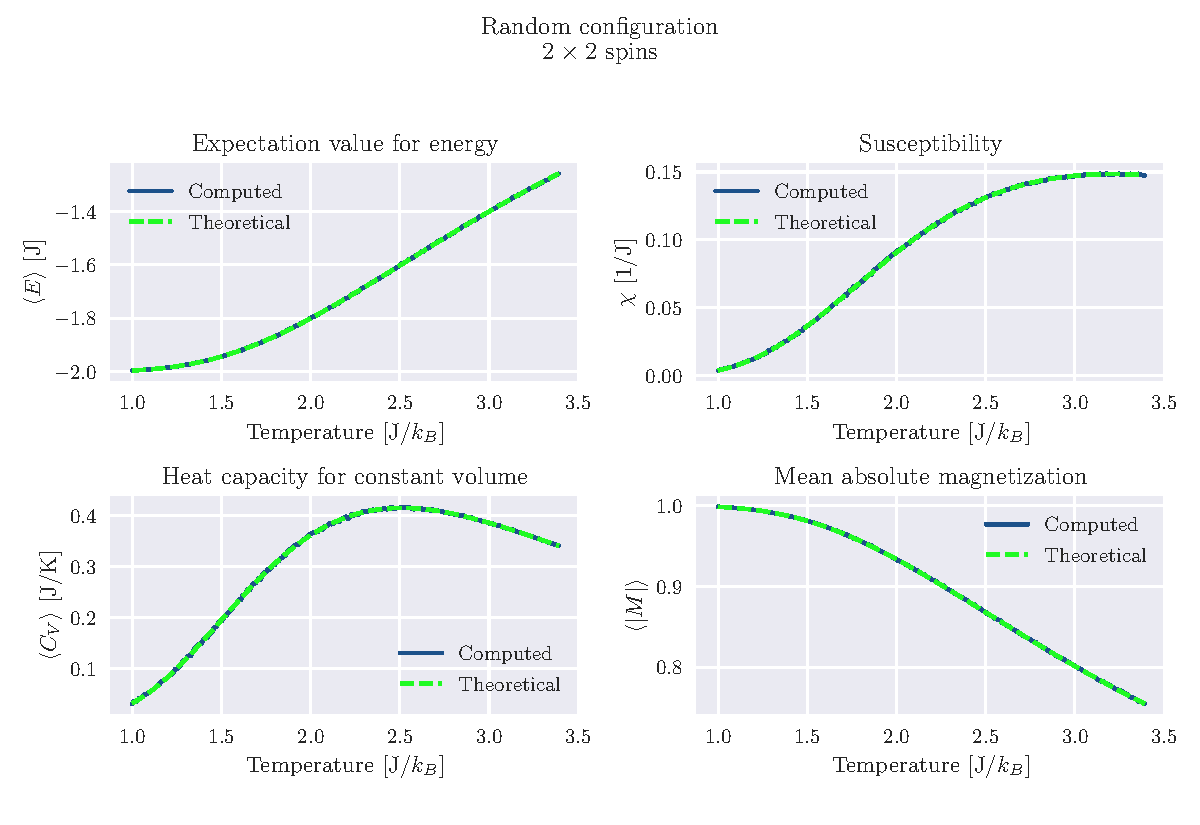
\includegraphics[width=\linewidth]{../output/c/L2-T1-dT0_01-NT240-N6-RandomFalse-CompTemp.pdf}
	\caption{In this figure you see the theoretical and computed values of $\left<E\right>$, $\left<|M|\right>$, $C_V$ and $\chi$, for a 2$\times$2 lattice. They are all plotted as a function of temperature, with random initial conditions.}
	\label{fig:L2_Random}
\end{figure*}
\section{Discussion}

From figure \ref{fig:L2_Random}, we se that the computed expectation values for a $2 \times 2$ lattice correspond extremely well with the theoretical values for temperatures $T \in [1.0, 3.5]$. When plotting for a specific temperature as a function Monte Carlo cycles, there was always what we could describe as a break-in time. Figure \ref{fig:L2_T1_Random_and_not} shows that we can potentially have large fluctuations during the first few thousand cycles. It seems that we can be fairly confident in our computed values after about 20 000 cycles. Notice that in figure \ref{fig:L2_T1_Random_and_not} the scales on the y-axes differ between the ordered and random configuration. The system in its ordered start configuration is already in or close to its equilibrium state from the start of the simulation and the expectation values never fluctuate far from the expected values. The relative error in energy is at most 0.2\% for the ordered start configuration and 3\% for the random start configuration. 100 000 Monte Carlo cycles seems sufficient to be confident that the relative error in our computed expectation values is low.

However, since our simulation is based on random sampling, we saw large differences in results from different runs of the code and they were not always as quick to converge as in figure \ref{fig:L2_T1_Random_and_not}. The random start configuration of the $2 \times 2$ lattice sometimes had a large effect on the results for tens of thousands of cycles. It seemed therefore that our algorithm is quite sensitive to random variations, but that we could count on convergence past 100 000 cycles.

Figure \ref{fig:L20_T1_and_T2_4} shows that the system converges on the same expectation values for all the properties with random and ordered configuration. The break-in period, where there are significant differences between the two lines only lasts for a few cycles for $T = 1$ J/$k_B$, and a few thousand cycles for $T = 2.4$ J/$k_B$. This corresponds to the initial steep rise of the graph of the top left plot in figure \ref{fig:Num_flips_T1_and_T2_4}. In the beginning of the simulation, very many spins are flipped because the system was initially far from its equilibrium state. When the system reaches its equilibrium state, the graph of the total number of flips is linear, which means that the number of flips per cycle is constant. Spins are flipped due to random, probabilistic fluctuations with the same frequency as long as the system is in its equilibrium state. The microstate changes as some spins flip from -1 to 1 and some flip from 1 to -1, but the macroscopic properties remain the same.



Looking at the histograms (figure \ref{fig:L20_prob_dist}) it does not seem to make any difference weather or not we have a ordered or random initial condition. The differences we do observe are not larger than what we see from run to run. We do however see a large difference for the two different temperatures. For temperature $T = 1$J/$k_B$ we see few and discrete possible values for energy. The values we observe do make sense, considering the possible energy differences we cover in the appendix. There are five possible changes in energy ($\Delta E$), $\Delta E = 0$J, $\Delta E = \pm 4$J and $\Delta E = \pm8$J. Accounting for total number of spins ($L^2 = 400$) and ignoring $\Delta E = 0$, that equates to four different changes in energy per spin, $\Delta E_s = \pm0.01$ and $\Delta E_s = \pm0.02$. With this in mind it is intuitive that we also should see a column for $E = -1.99$J and a larger column for $E = -1.97$J. However if we study the spin orientations in the appendix we notice that $E=1.99$J is impossible and $E = 1.97$J is unlikely. When we are in ground state (all spins pointing in one direction) the only possible change in energy is $\Delta E_s=0.02$J. From there we notice that the only possible changes are $\Delta E_s = \pm 0.02$J and $\Delta E = 0.01$J, not $\Delta E = -0.01$. This means $E = -1.99$J is impossible. Furthermore the only way we can get $\Delta E_s=0.01$J is by changing the neighboring spin of the one we just changed. This is unlikely, and therefore we see few situations of that happening. For the temperature $T = 2.4$J/$k_B$ the result looks Gaussian, and we therefore plotted a fit on top. The variance from the fit is the same as the one we computed. This does not surprise us, because we used the same data to calculate both values. It is interesting however that the probability-density distribution has a Gaussian shape, although it is difficult to say why. We expected to see a larger spectra for observed energies however. When we look at the equation that describes probability of flip (equation \eqref{eq:prob_flip}), in the exponent, temperature is in the denominator, meaning the probability for a flip gets higher overall.
eksluderte = fjerne 50 \%
kjør lengre =

The simulations giving us the results in figure \ref{fig:phase_trans} are quite costly and time consuming for large lattices. We are therefore limited in our resolution of temperature, which makes it impossible to determine the critical temperature $T_C$ exactly. But we can still read some useful information from the figure.

Theoretically, we expect the magnetization to go from non-zero to zero with a vertical slope at $T_C$. This clearly does not happen, but the tendency is there and we can identify the steepest slope on the graph showing absolute magnetization. For $L = 100$ this seems to be at a temperature just under 2.3 J/$k_B$. For smaller lattices, it seems to be shifted ever so slightly towards higher temperatures. At the same temperature we find the steepest slope of the energy graph and the peak the heat capacity graph. The peak of heat capacity is located at $T_C = 2.28$ J/$k_B$, which is definitely in the neighborhood of Lars Onsager's critical temperature of $kT_C/\rm{J} \approx 2.269$.

As the peaks of heat capacity and susceptibility are higher for $L = 100$ than for lower values of $L$, we believe that the true peak is closer to 2.28 J/$k_B$ for $L = 100$ than for lower values of $L$. With our limited resolution, the peaks seem lower because the temperature of the true peak may be ''hidden'' between two of our temperature grid values at for instance 2.29 J/$k_B$. This is illustrated in figure \ref{fig:drawing_critical_temp}. As the peaks and steepest points of the graphs are slightly shifted to the right for smaller values of $L$, still seems plausible. We therefore also believe the critical temperature would continue to approach Onsager's value of 2.269 J/$k_B$ for values of $L$ larger than 100.
\begin{figure}
  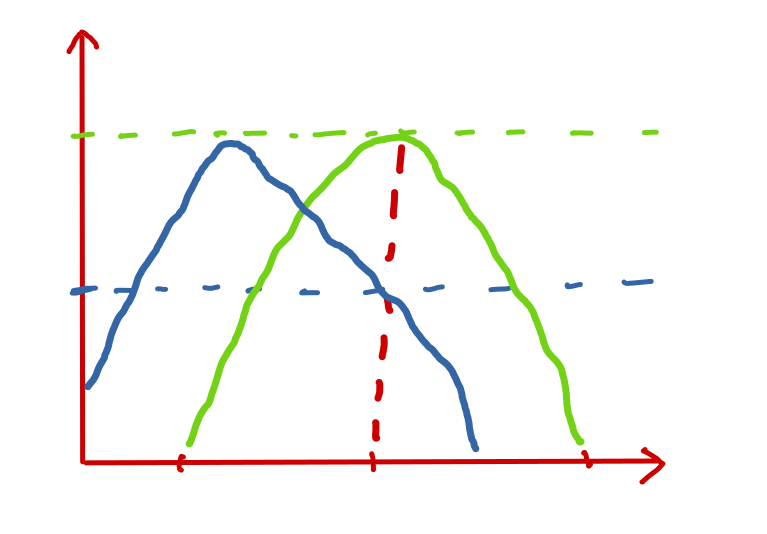
\includegraphics[width=\linewidth]{../output/Drawing.png}
  \caption{An illustration of}
  \label{fig:drawing_critical_temp}
\end{figure}

In order to determine the critical temperature more precisely, we could rerun the simulations for a narrower range of temperatures. We now know $T_C$ to be close to 2.3 J/$k_B$, and it is not necessary to cover temperatures from 2.0 J/$k_B$ to 2.5 J/$k_B$ in every simluation. It is useful to start width a wide range of values for the temperature to show the big picture like we have done here. To further develop our results, narrowing the range of $T$ and increasing the resolution would clearly be a natural first step.


General improvements: axis fix, burn-in time

\section{Conclusion}

\section{Appendix}
\subsection{Algorithm specific optimization}

In order to make our algorithm run faster, we do some optimization. We list the optimizations we implemented here, to make our code easier to understand and as a guide for anyone who wants to do something similar.

During our simulations we calculate the change in energy ($\Delta$E) many times. We want to make more efficient by exploring the possible values $\Delta E$ can have. During our simulations we only evaluate one spin at a time, meaning we only need to look at the possible values $\Delta E$ can have when flipping one spin. It turns out there are five possible situations (using equation \eqref{eq:2D_energy}):
\begin{align*}
	\text{Zero down: } &\begin{matrix}
	& \uparrow  \\
	\uparrow & \uparrow & \uparrow \\
	& \uparrow
	\end{matrix}
	\rightarrow
	\begin{matrix}
	& \uparrow  \\
	\uparrow & \downarrow & \uparrow \\
	& \uparrow
	\end{matrix}
	\implies
	\Delta E = 8J \\
	\text{One down: }
		&\begin{matrix}
	& \downarrow  \\
	\uparrow & \uparrow & \uparrow \\
	& \uparrow
	\end{matrix}
	\rightarrow
	\begin{matrix}
	& \downarrow  \\
	\uparrow & \downarrow & \uparrow \\
	& \uparrow
	\end{matrix}
	\implies
	\Delta E = 4J \\
	\text{Two down: }
		&\begin{matrix}
	& \downarrow  \\
	\downarrow & \uparrow & \uparrow \\
	& \uparrow
	\end{matrix}
	\rightarrow
	\begin{matrix}
	& \downarrow  \\
	\downarrow & \downarrow & \uparrow \\
	& \uparrow
	\end{matrix}
	\implies
	\Delta E = 0J \\
	\text{Three down: }
		&\begin{matrix}
	& \downarrow  \\
	\downarrow & \uparrow & \downarrow \\
	& \uparrow
	\end{matrix}
	\rightarrow
	\begin{matrix}
	& \downarrow  \\
	\downarrow & \downarrow & \downarrow \\
	& \uparrow
	\end{matrix}
	\implies
	\Delta E = -4J \\
	\text{Four down: }
		&\begin{matrix}
	& \downarrow  \\
	\downarrow & \uparrow & \downarrow \\
	& \downarrow
	\end{matrix}
	\rightarrow
	\begin{matrix}
	& \downarrow  \\
	\downarrow & \downarrow & \downarrow \\
	& \downarrow
	\end{matrix}
	\implies
	\Delta E = -8J \\
\end{align*}
We can thus compute and store the different values of $e^{- \frac{\Delta E}{k_BT}}$ beforehand to avoid making these computations every time we update the energy.

As mentioned previously, we are going to use periodic boundary conditions. The easiest, but slow way of implementing this, is with if-tests. However we did it with a simple function (in c++),
\begin{lstlisting}
int PeriodicBoundary(int i, int limit, int add) {
	return (i+limit+add) % (limit);
}
\end{lstlisting}
that takes the current index you are evaluating (\texttt{i}), the total size (\texttt{limit}) and the amount you want to go forward and backward (\texttt{add}). Then we sum all the arguments and take the rest, reassuring us that we always arrive at the right index.

When we run our simulations for different temperatures, for example when studying phase transitions, we ended up parallelizing our code. The different temperatures are not dependant on eachother, so we can allocate the task to different cores. This was easiliy done with OpenMP.

\subsection{Calculations of 2$\times$2 lattice} \label{calc_of_22_lattice}

Inserting the values from table \ref{tab:E_and_M_2D_lattice} into equations \eqref{eq:canonical_ensemble} and (\ref{eq:expected_energy}-\ref{eq:specific_heat_capacity}) we get
\begin{align*}
	\left<E\right> &= \frac{1}{Z}\left(-8Je^{8\beta} + 2\cdot 8Je^{-8\beta } - 8J e^{8\beta }\right) \\
	&= \frac{-32J}{Z}\cosh(8\beta )\\
	\left<E^2\right> &= \frac{1}{Z}\left((-8J)^2e^{8\beta J} + 2\cdot (8J)^2e^{-8\beta J} (- 8J)^2 e^{8\beta }\right) \\
	&= \frac{256J^2}{Z}\cosh(8\beta)\\
	\left<|M|\right> &= \frac{1}{Z}\left(4e^{8\beta } + 4\cdot 2e^{0} + 4\cdot 2 e^{0} + 4e^{8\beta }\right) \\
	&= \frac{8}{Z}\left(2 + e^{8\beta }\right)\\
	\left<M^2\right> &= \frac{1}{Z}\left(4^2e^{8\beta } + 4\cdot 2^2e^{0} + 4\cdot 2^2 e^{0} + 4^2e^{8\beta }\right) \\
	&= \frac{32}{Z}\left(1 + e^{8\beta }\right)\\
	\chi &= \frac{32\beta}{Z}\left(\left(1 + e^{8\beta }\right) - \frac{2}{Z}\left(2 + e^{8\beta }\right)^2 \right)\\
	C_V &= \frac{256J^2\beta}{TZ}\left(\cosh(8\beta) - \frac{4}{Z}\cosh[2](8\beta)\right)
\end{align*}

\begin{figure*}[!htb]
	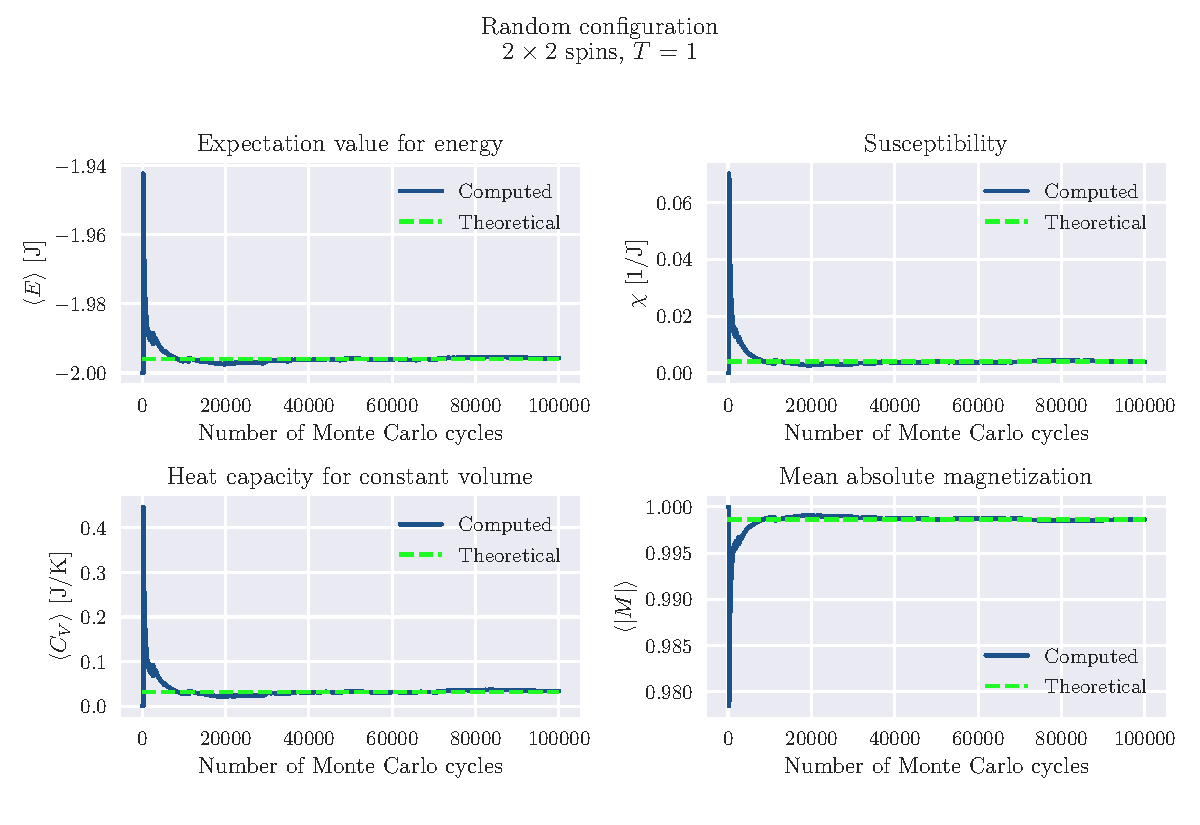
\includegraphics[width=16cm]{../output/c/L2-T1-dT0_0-NT1-N5-RandomTrue-CompCycle.pdf}
	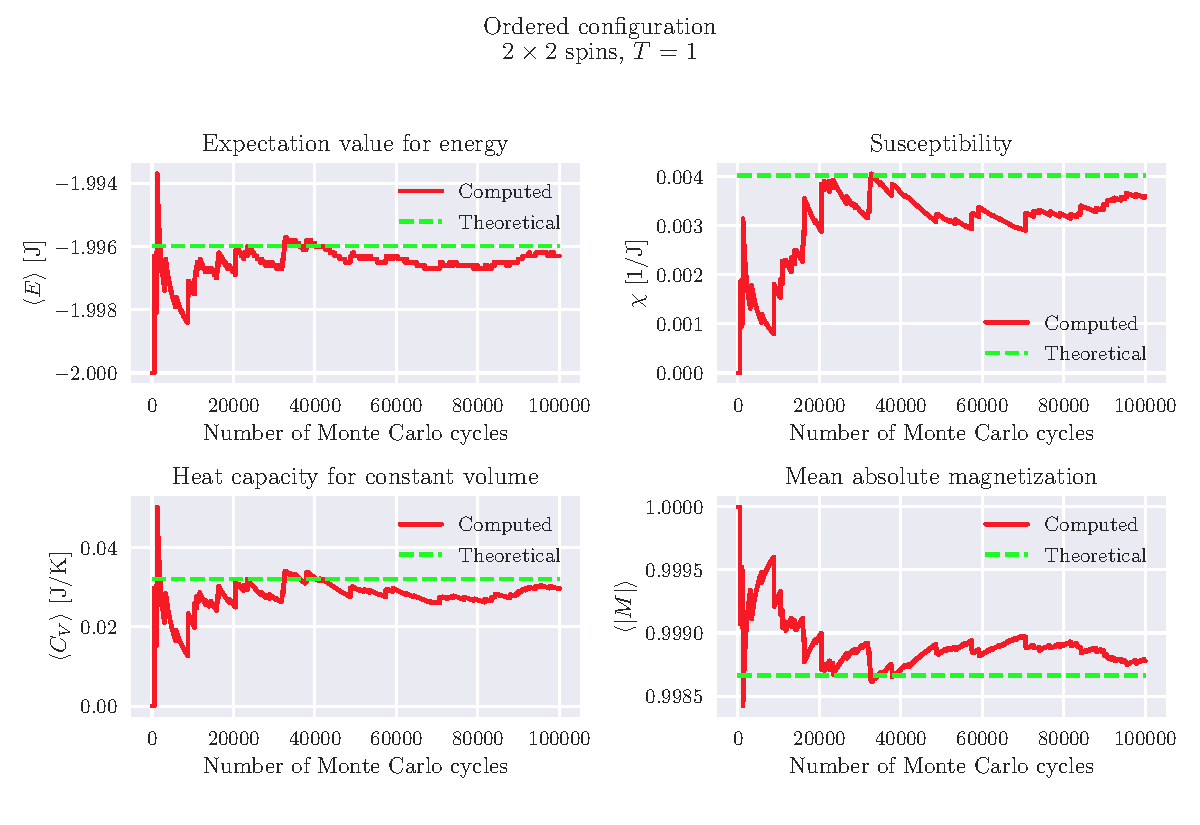
\includegraphics[width=16cm]{../output/c/L2-T1-dT0_0-NT1-N5-RandomFalse-CompCycle.pdf}
	\caption{In this figure you see the theoretical and computed values of $\left<E\right>$, $\left<|M|\right>$, $C_V$ and $\chi$, for a 2$\times$2 lattice and temperature $T=1\rm{J}/k_B$. The top four plots are from random initial values, and the bottom four have ordered initial conditions.}
	\label{fig:L2_T1_Random_and_not}
\end{figure*}
\begin{figure*}[!htb]
	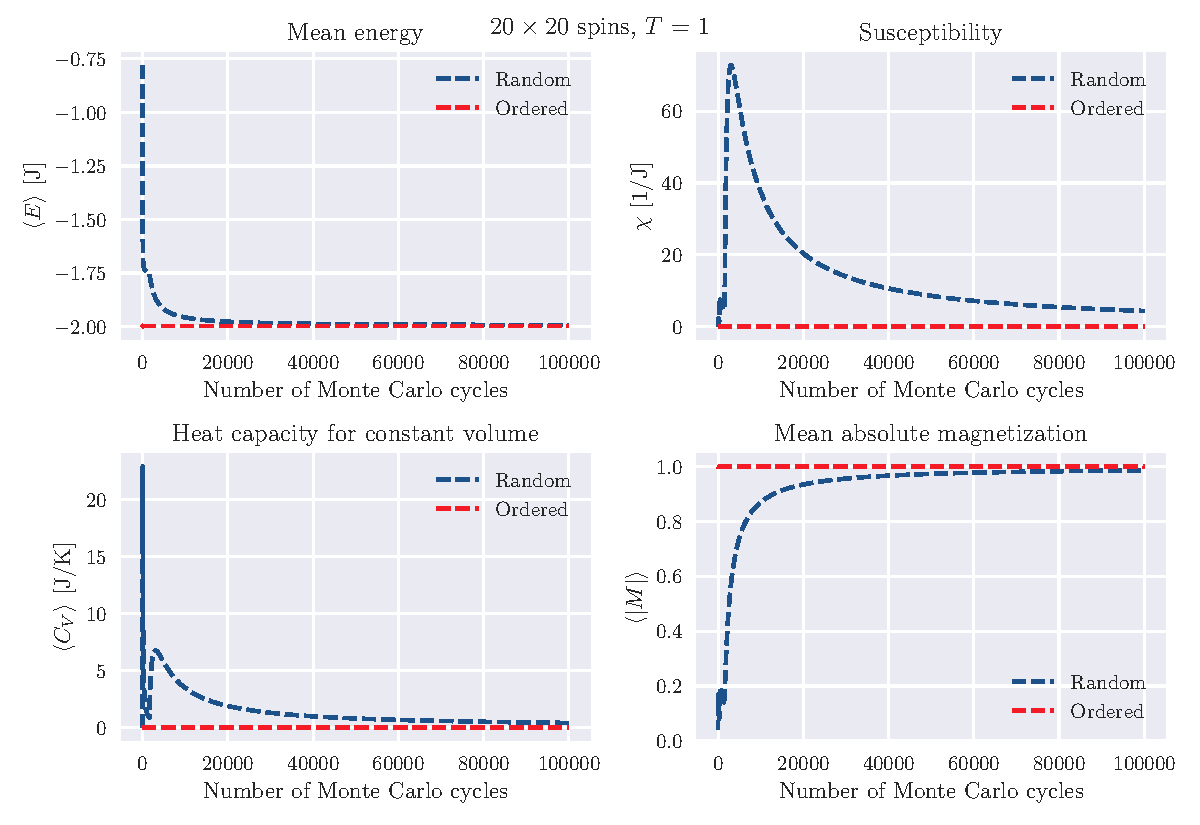
\includegraphics[width=16cm]{../output/de/L20-T1-dT0_0-NT1-N5-ExpVals.pdf}
	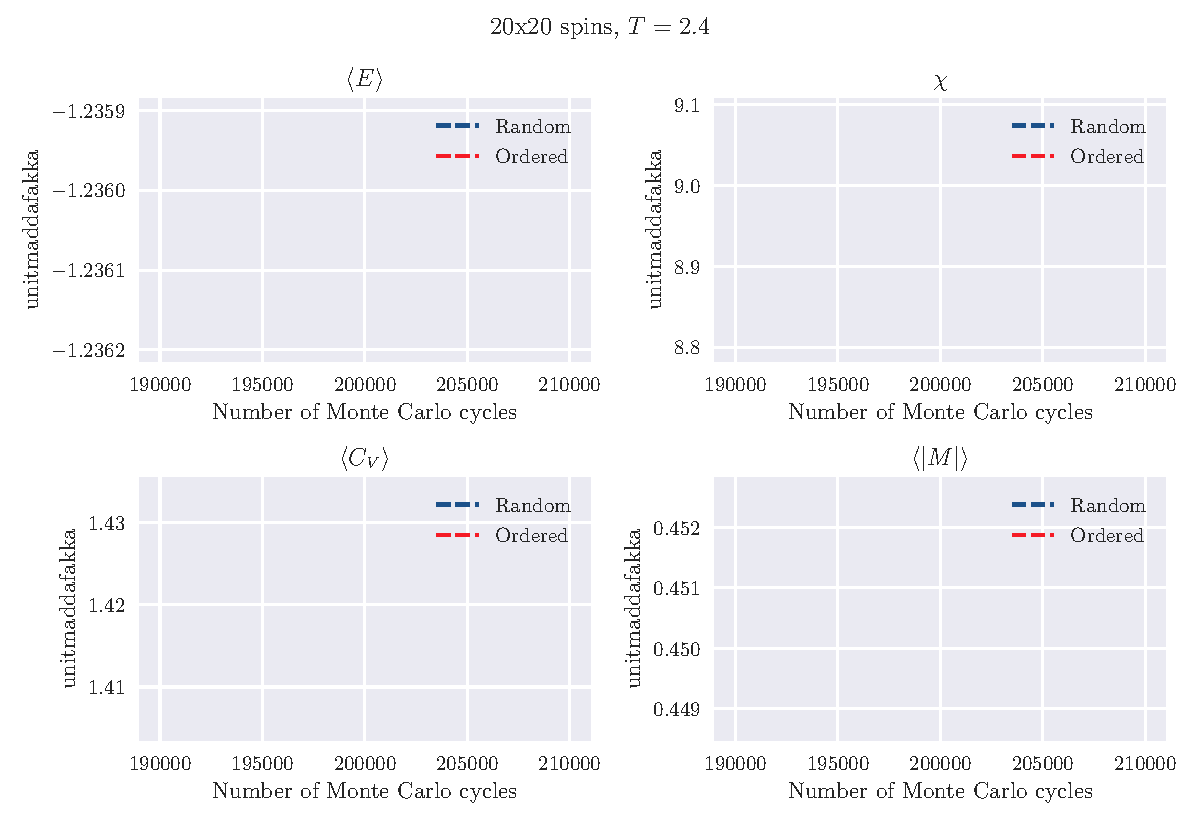
\includegraphics[width=16cm]{../output/de/L20-T2_4-dT0_0-NT1-N5-ExpVals.pdf}
	\caption{In this figure you see the computed values of $\left<E\right>$, $\left<|M|\right>$, $C_V$ and $\chi$, for both random and ordered initial conditions. The top four shows the computed values for random and ordered initial conditions, for a temperature $T=1\rm{J}/k_B$. Bottom four shows the same, only for a temperature $T=2.4\rm{J}/k_B$.}
	\label{fig:L20_T1_and_T2_4}
\end{figure*}
\begin{figure*}[!htb]
	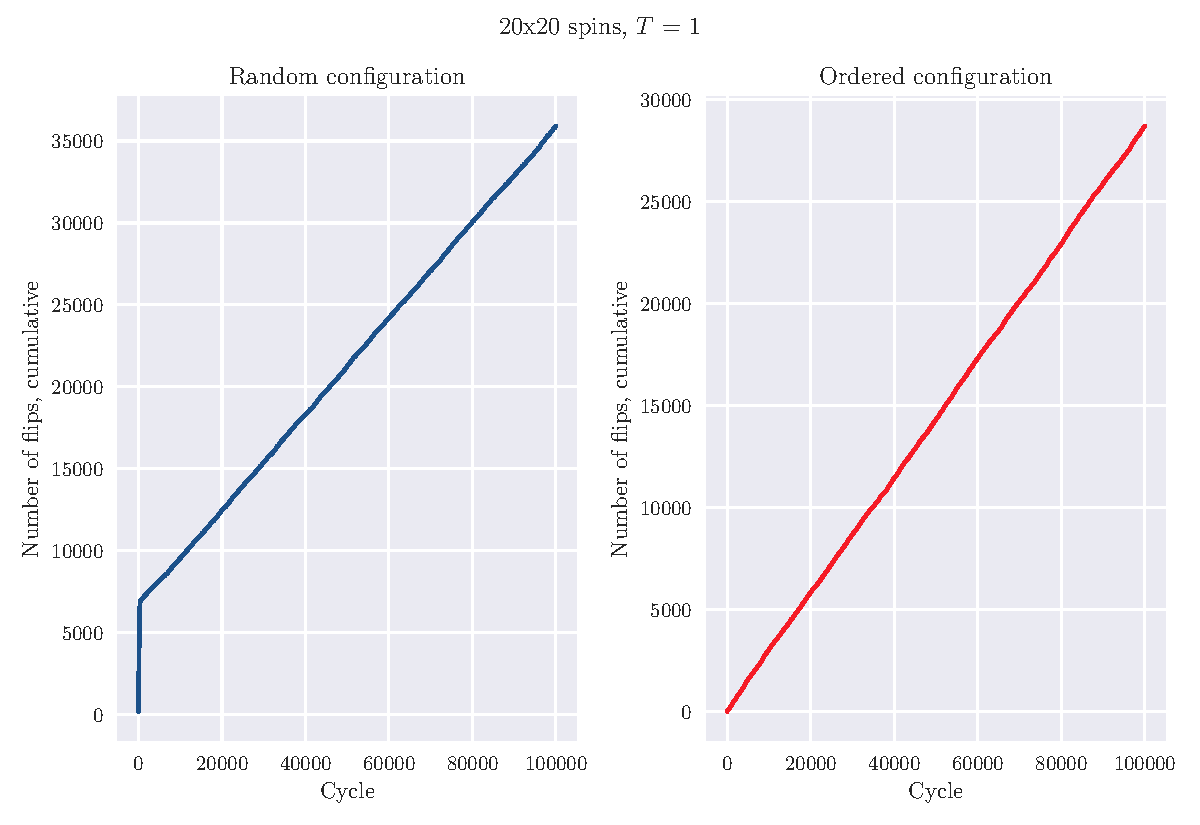
\includegraphics[width=16cm]{../output/de/L20-T1-dT0_0-NT1-N5-NumFlips.pdf}
	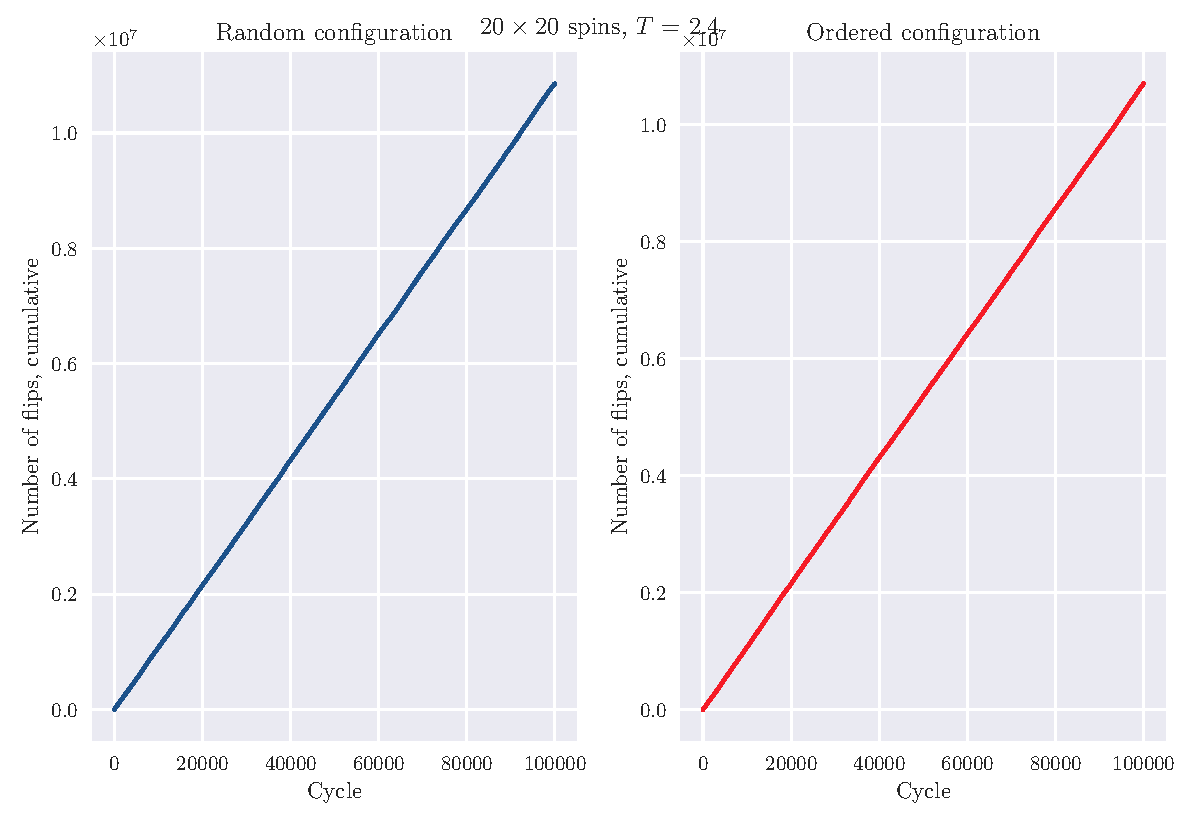
\includegraphics[width=16cm]{../output/de/L20-T2_4-dT0_0-NT1-N5-NumFlips.pdf}
	\caption{Here we have plotted the number of accepted configuration as a function of Monte Carlo cycles, for a 20$\times$20 lattice. The top two plots are with temperature $T=1\rm{J}/k_B$, and shows both random and ordered initial conditions. The bottom two shows the same, only with a temperature of $T = 2.4\rm{J}/k_B$.}
	\label{fig:Num_flips_T1_and_T2_4}
\end{figure*}
\begin{figure*}[!htb]
	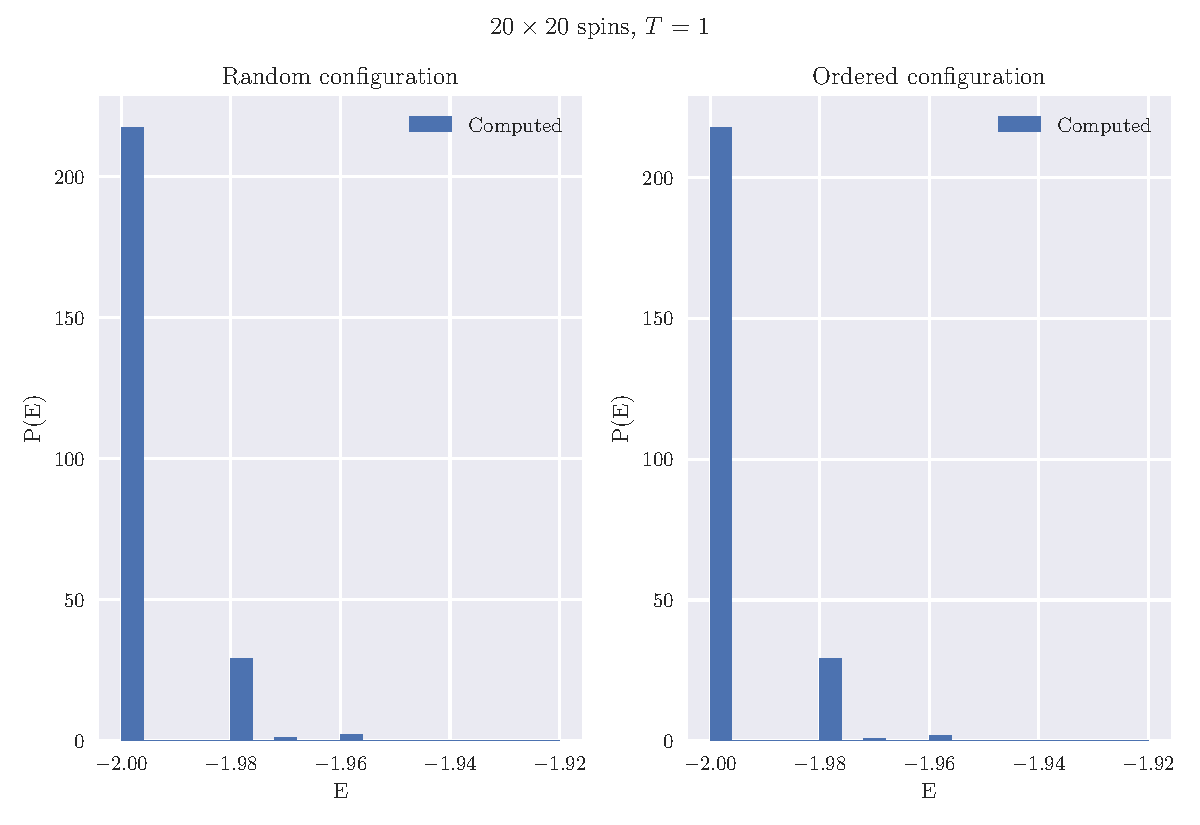
\includegraphics[width=16cm]{../output/de/L20-T1-dT0_0-NT1-N5-ProbE.pdf}
	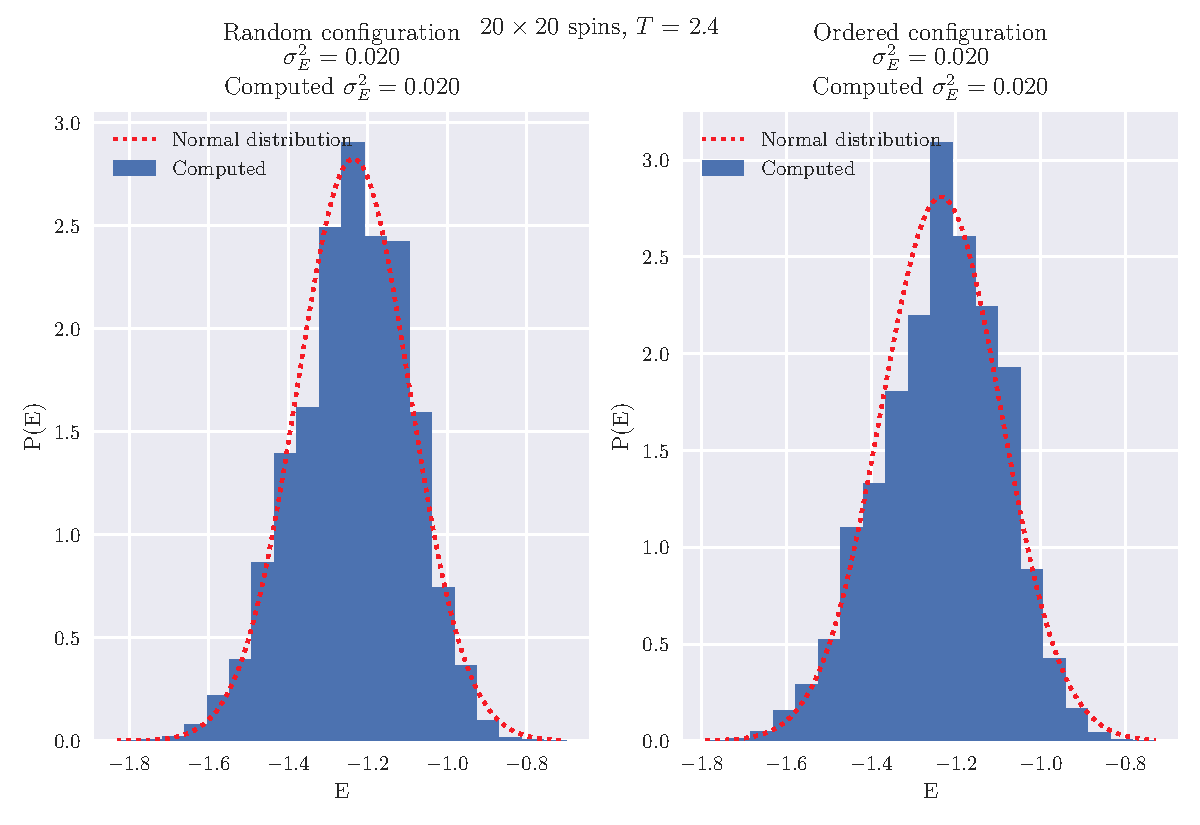
\includegraphics[width=16cm]{../output/de/L20-T2_4-dT0_0-NT1-N5-ProbE.pdf}
	\caption{These histograms shows the probability density of a given energy. The top two plots are for $T = 1$J/$k_B$ with ordered and random inital conditions. The bottom two are for $T = 2.4$J/$k_B$, also with random and ordered initial conditions. We have also done a gaussian fit to the bottom results (the red dotted graph). In the title you see the variance of our data ($\sigma_E$), and below the variance we computed with our simulations.}
	\label{fig:L20_prob_dist}
\end{figure*}
\begin{figure*}[!htb]
	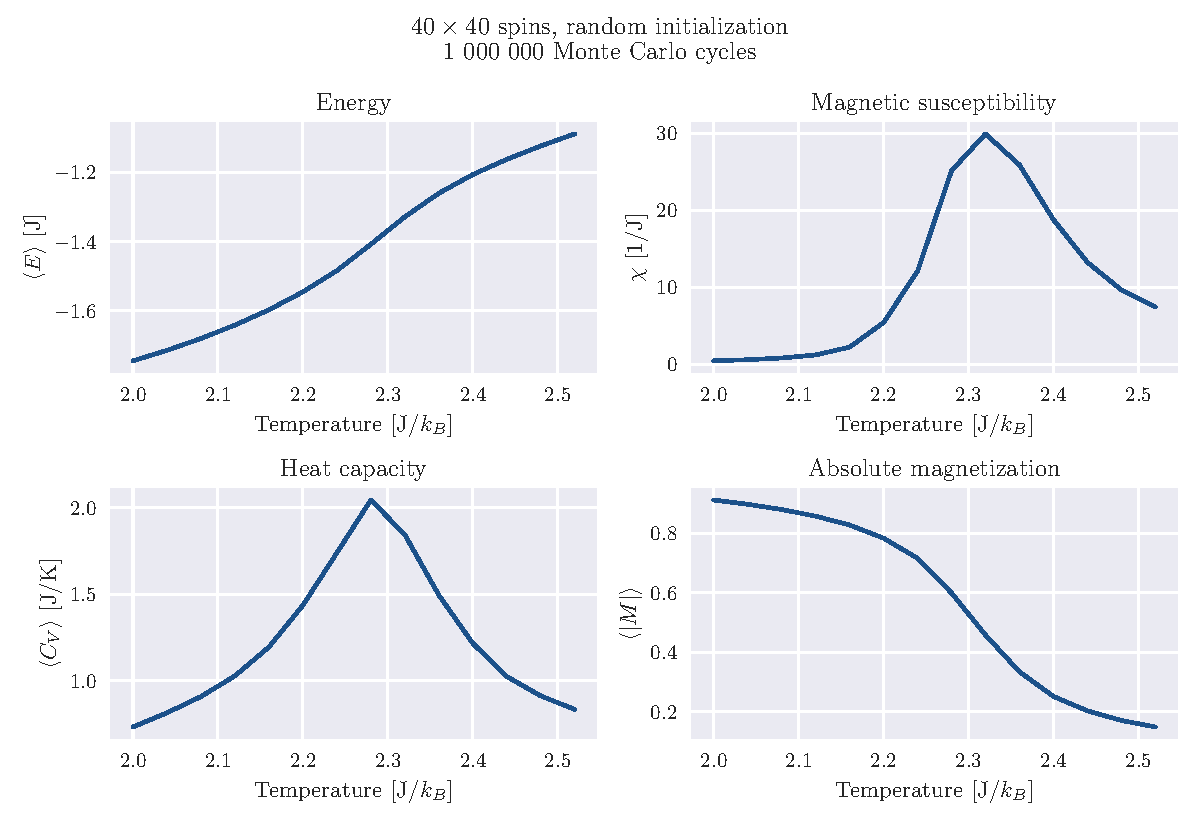
\includegraphics[width=16cm]{../output/f/L40-T2_0-dT0_04-NT14-N6-RandomTrue-TempExp.pdf}
	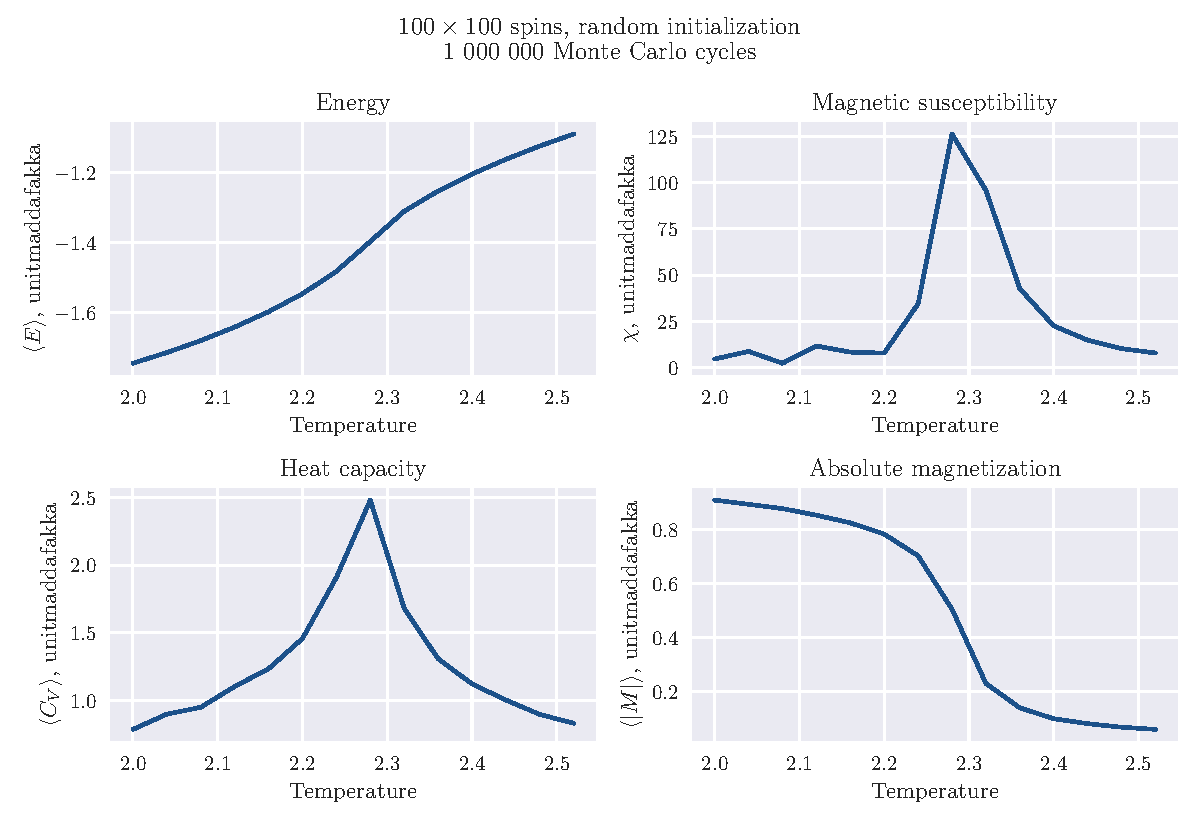
\includegraphics[width=16cm]{../output/f/L100-T2_0-dT0_04-NT14-N6-RandomTrue-TempExp.pdf}
	\caption{Here we have plotted the computed values of $\left<E\right>$, $\left<|M|\right>$, $C_V$ and $\chi$, as a function of temperature. The top four are for a 40$\times$40 lattice with random initial conditions, and the bottom four are from a 100$\times$100 lattice, also with random initial conditions.}
	\label{fig:phase_trans}
\end{figure*}



\onecolumngrid
\vspace{1cm} % some extra space

\begin{thebibliography}{}
\bibitem[]{lectures2015} Morten Hjorth-Jensen, Computational Physics, Lecture Notes Fall 2015, August 2015, https://github.com/CompPhysics/ComputationalPhysics/blob/master/doc/Lectures/lectures2015.pdf.
\bibitem[]{larsonsager} Lars Onsager, Crystal Statistics. I. A two-Dimensional Model with an Order-Disorder Transition, 1. February 1944, https://journals.aps.org/pr/abstract/10.1103/PhysRev.65.117

\end{thebibliography}


\end{document}
